\section{Other agent architectures}
\label{sec:patterns}

The previous sections took \msa{} through a fixed workflow, a reactive loop (ReAct), a planner and
a validator. Each time, the agent, the alert and the tools stayed the same, so only the
architecture changed. We now survey further architectures from a published catalogue of agentic
design patterns. We sort them by who orchestrates them, that is, by who decides which component
runs next. The answer determines whether we can read the order of a run from the program. It also
shapes what a pattern costs and how easily we can find its mistakes.

\subsection{Design patterns and who orchestrates them}
\label{sec:patterns-catalogue}

An \textbf{agentic design pattern} is a reusable arrangement of model calls, agents and the logic
that connects them, described independently of any particular task. A published catalogue
describes twelve such patterns \citep{google2026patterns}, and we study eleven of them.

Each pattern describes an agent architecture in the sense of the previous sections: it fixes which
components exist and who decides what runs next. A model call is a single request to a model and
its reply. In these patterns, an agent is a component built around a model. It may make several
model calls, and often use tools, to finish its part of the work.

Several of the patterns use more than one agent, so we name the roles an agent can play inside a
larger system:
\bi
\item \textbf{Subagent.} A subagent is an agent that another agent, or the program that runs the
agents, calls to carry out one part of the task.
\item \textbf{Specialist.} A specialist is a subagent built for one kind of work.
\item \textbf{Worker.} A worker is a subagent that carries out its part of the task directly,
without dividing it further.
\ei

\textbf{Orchestration} is the work of deciding which component runs next, what input it receives,
and when the task is finished. These are control decisions, the decisions that determine how a run
proceeds (\cref{sec:fixed-definition}). The component that makes them is the orchestrator, the
component that Unit~1 of the course studies (\cref{sec:logistics}).

We sort the patterns by who orchestrates them. Most patterns fall on one side of a single division:
either a model orchestrates, or predefined logic does. The remaining patterns give other answers.

\textbf{Predefined logic} is code, written at design time, that arranges the components in a fixed
structure. The structures in the catalogue are a sequence, a set of workers whose results are
gathered, and a loop. Predefined logic fixes
which components run, how they are arranged and what ends the work, as the steps of a fixed
workflow are fixed (\cref{sec:fixed}). When a model orchestrates, it makes these decisions at run
time from what it has read, as the model in a reactive loop chooses each next action
(\cref{sec:reactive}).

The eleven patterns we study answer the question of who orchestrates as follows:
\bi
\item \textbf{The model.} A model orchestrates the reason and act pattern, the coordinator pattern
and the hierarchical task decomposition pattern. In reason and act, the model works inside a single
agent. In hierarchical task decomposition, models orchestrate at several levels.
\item \textbf{Predefined logic.} Predefined logic orchestrates the sequential, parallel and loop
patterns. It also runs the review and critique pattern and the iterative refinement pattern as
loops.
\item \textbf{Predefined checkpoints.} In the human-in-the-loop pattern, the run stops at points
fixed at design time and waits for a person to decide. A checkpoint here is such a pause for a
person's decision. It differs from the checkpoint that saves a run's progress so that the run can
resume (\cref{sec:fixed-parts}).
\item \textbf{Code the team writes.} In the custom logic pattern, the team that builds the system
writes its own conditional code, which combines the other patterns.
\item \textbf{No central orchestrator.} In a swarm, no single component decides what runs next.
\ei

The answer matters because it determines which control decisions are known before a run starts.
When predefined logic orchestrates, we can read the possible orders of execution from the program,
as we could for a fixed workflow. When a model orchestrates, the order is chosen during the run.
Only the run's trace, the log of events that the runtime writes during a run
(\cref{sec:reactive-edge}), then shows what was chosen.

Some of the patterns restate architectures we have already studied. The reason and act pattern is
the reactive loop of \cref{sec:reactive}. The sequential pattern has the shape of a fixed workflow.
The review and critique pattern separates the component that proposes a result from the component
that accepts it, as the validator does (\cref{sec:validation}).

\Cref{fig:patterns-react-to-refinement} shows the first six patterns as the catalogue draws them.
In each diagram, the user's prompt enters on the left, and the arrows show which components run and
in what order. In the reason and act diagram, the memory box plays the role of the run's state.
Each observation is saved there, and the next thought reads it.

In the sequential, parallel and loop diagrams, the box that receives the prompt is labeled an agent
(sequential agent, parallel agent, loop agent). That box is the predefined logic. It runs its
subagents in an arrangement written before the run, and no model decides the order. In the
diagrams of the review and critique pattern and the iterative refinement pattern, the generator is
labeled a loop agent. The label shows that the generator runs inside a loop that predefined logic
controls.

\begin{figure*}[t]
  \centering
  \begin{subfigure}[b]{0.8\textwidth}
    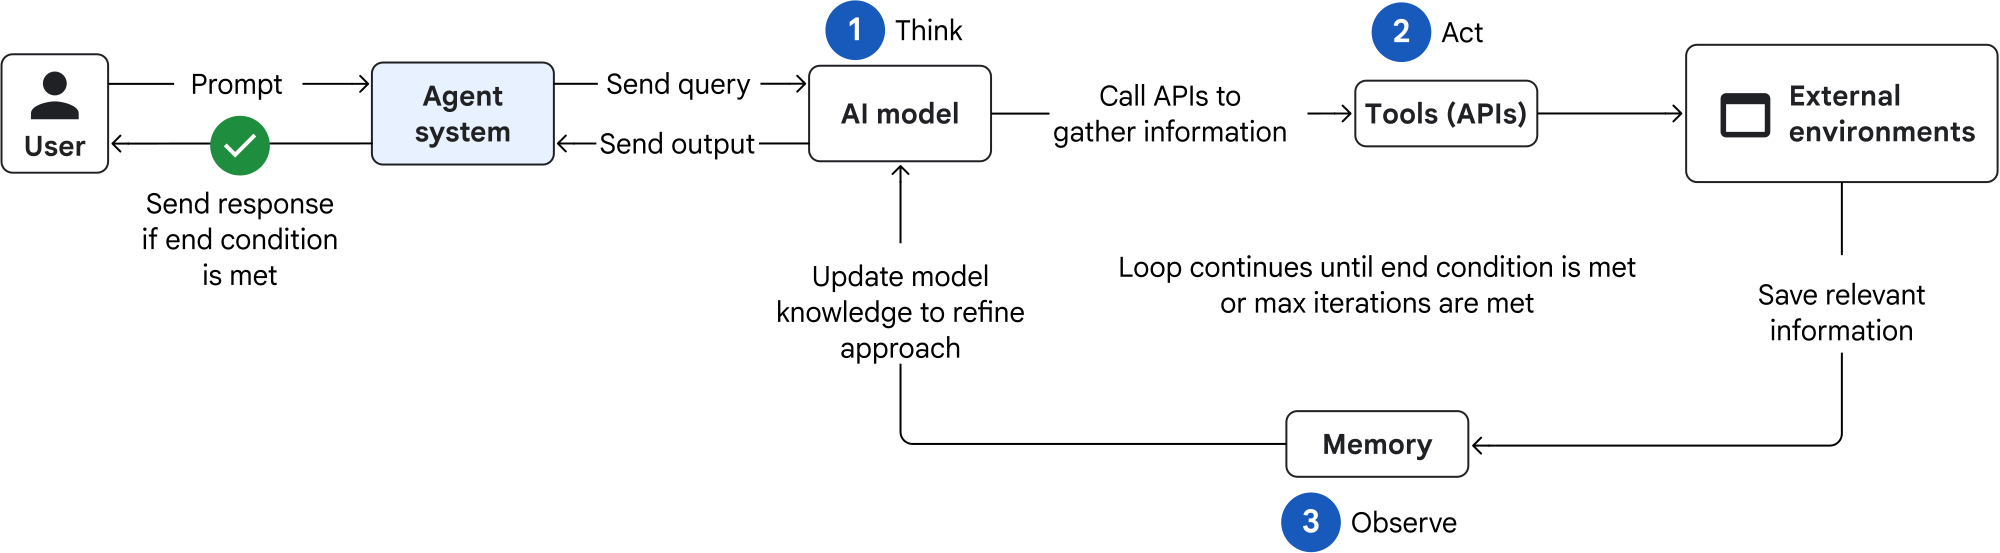
\includegraphics[width=\linewidth]{figures/deck/gcp-reason-and-act.png}
    \caption{Reason and act}
    \label{fig:patterns-react}
  \end{subfigure}

  \medskip
  \begin{subfigure}[b]{0.6\textwidth}
    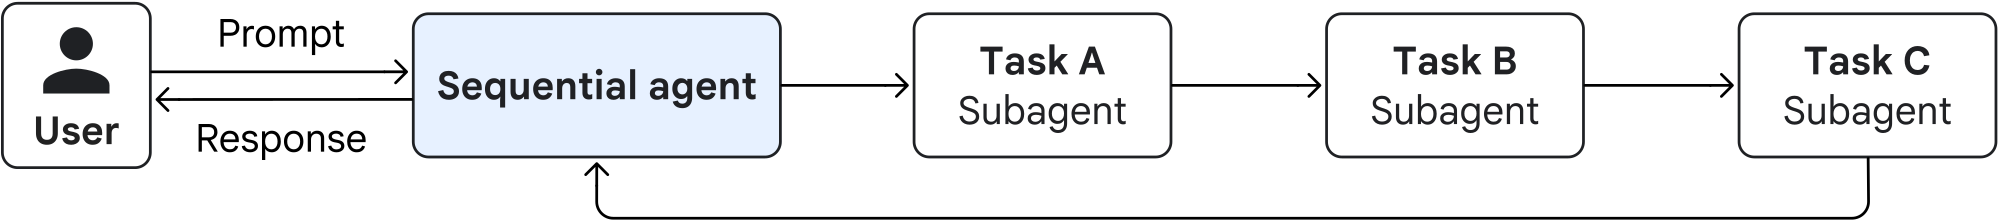
\includegraphics[width=\linewidth]{figures/deck/gcp-sequential.png}
    \caption{Sequential}
    \label{fig:patterns-sequential}
  \end{subfigure}

  \medskip
  \begin{subfigure}[b]{0.32\textwidth}
    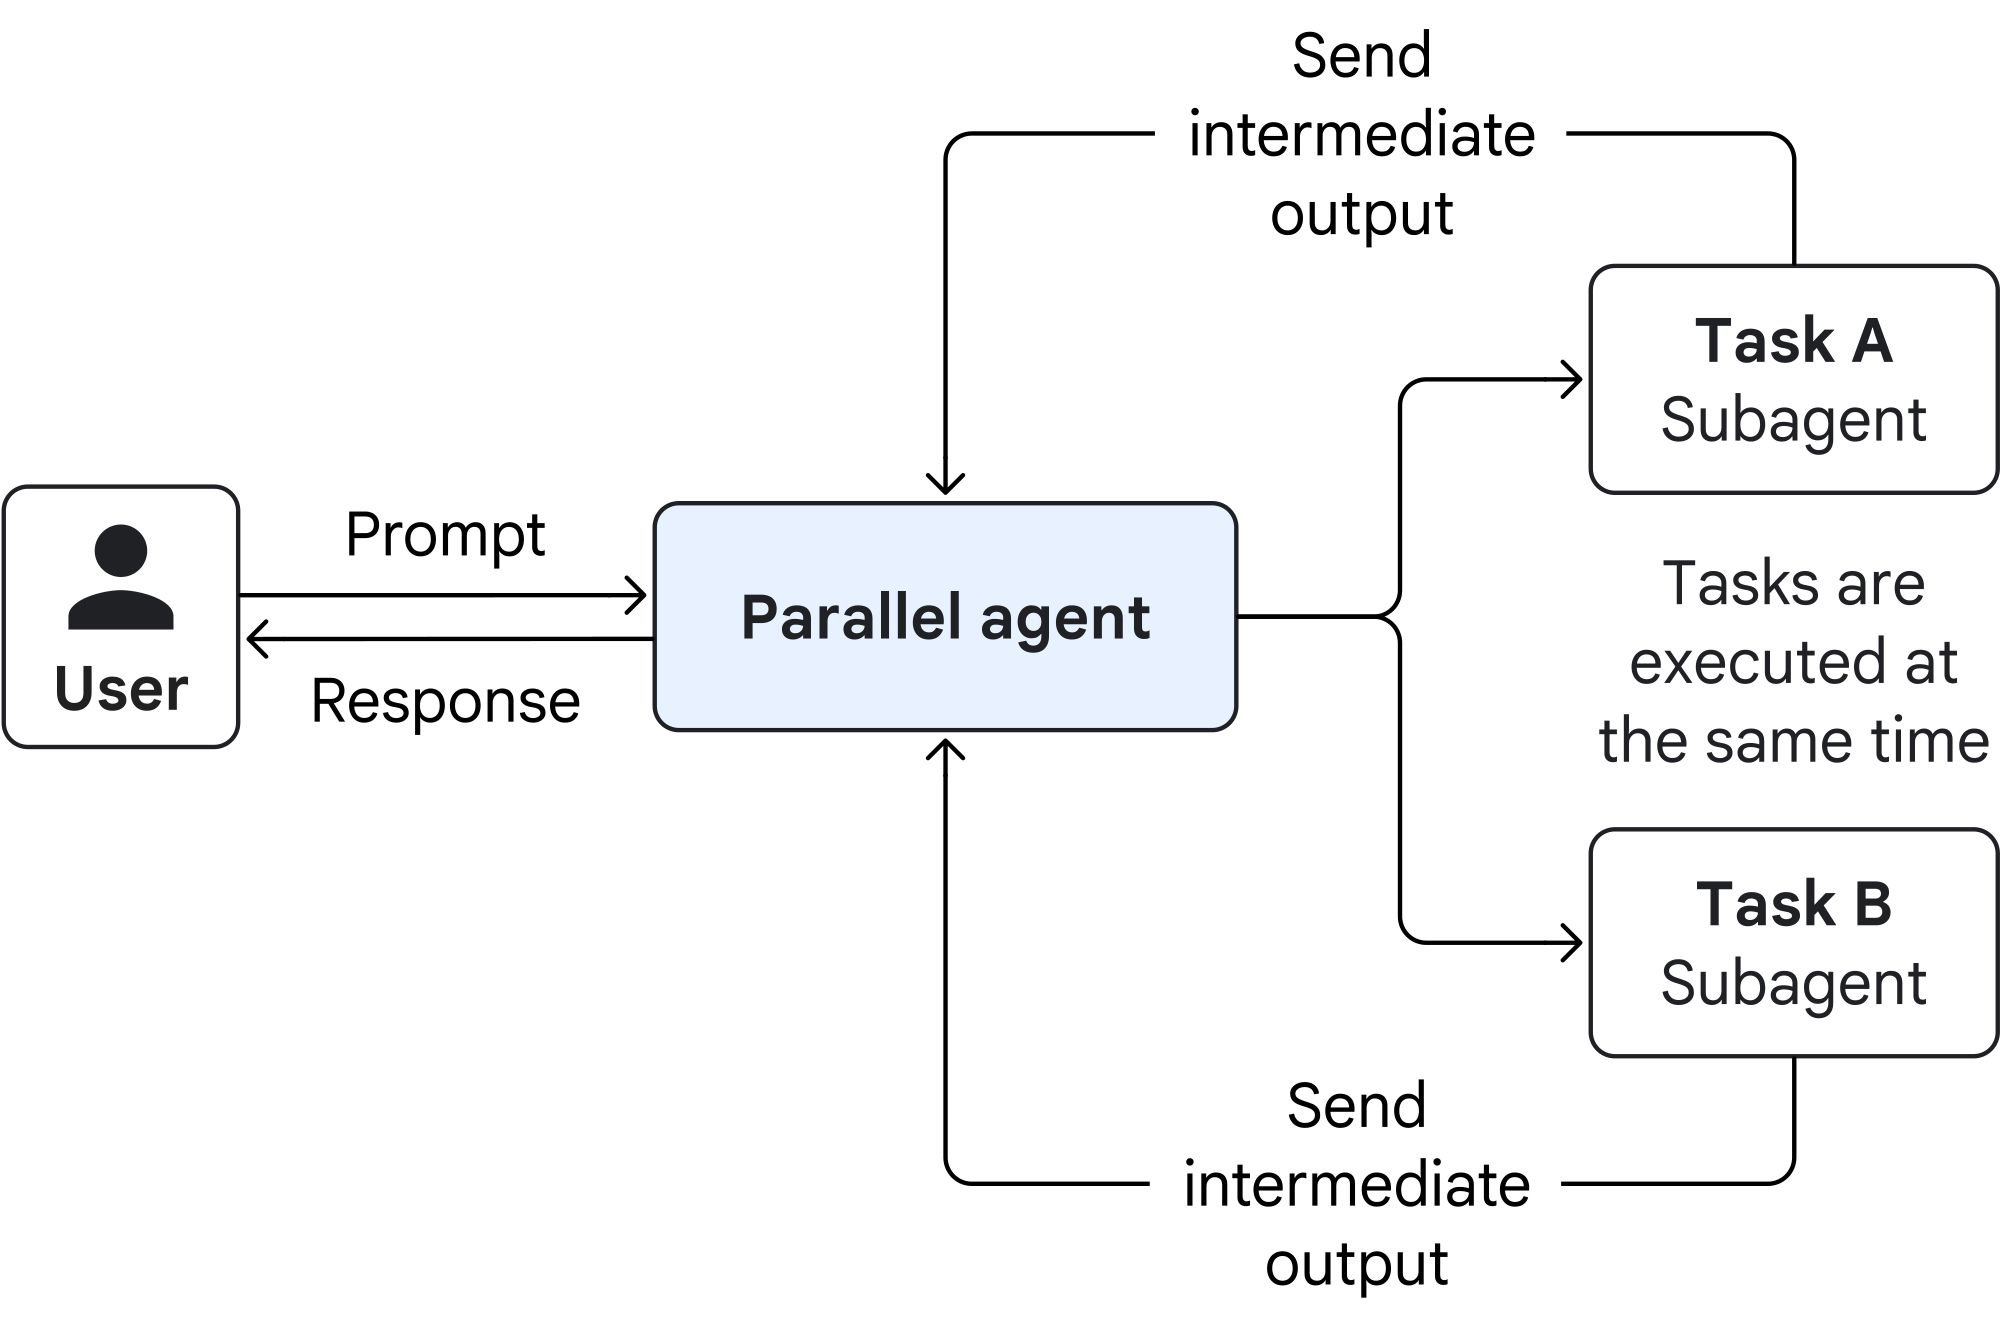
\includegraphics[width=\linewidth]{figures/deck/gcp-parallel.png}
    \caption{Parallel}
    \label{fig:patterns-parallel}
  \end{subfigure}\hfill
  \begin{subfigure}[b]{0.62\textwidth}
    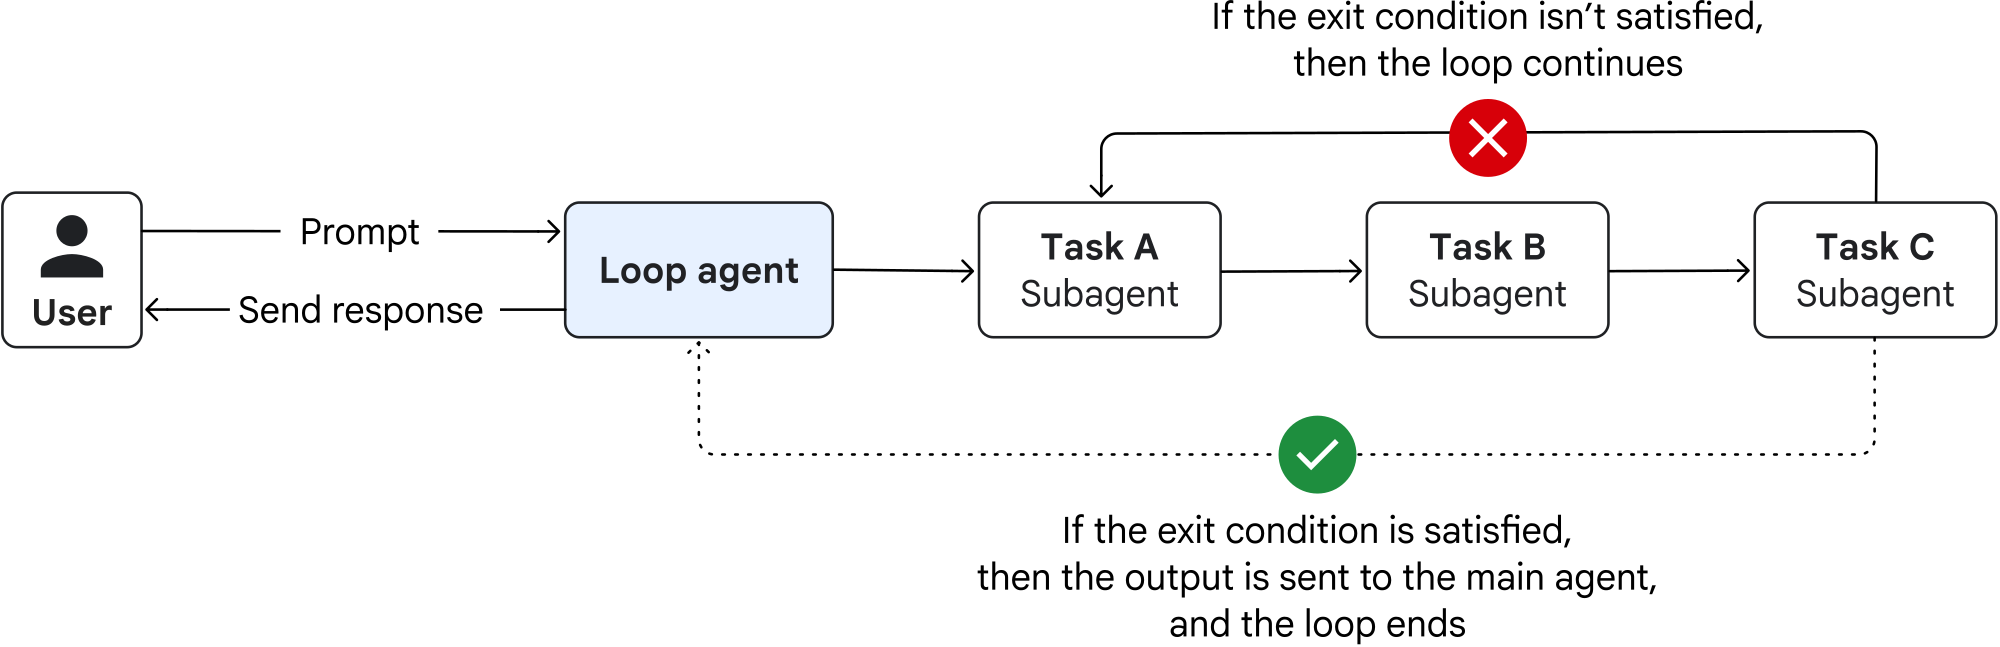
\includegraphics[width=\linewidth]{figures/deck/gcp-loop.png}
    \caption{Loop}
    \label{fig:patterns-loop}
  \end{subfigure}

  \medskip
  \begin{subfigure}[b]{0.48\textwidth}
    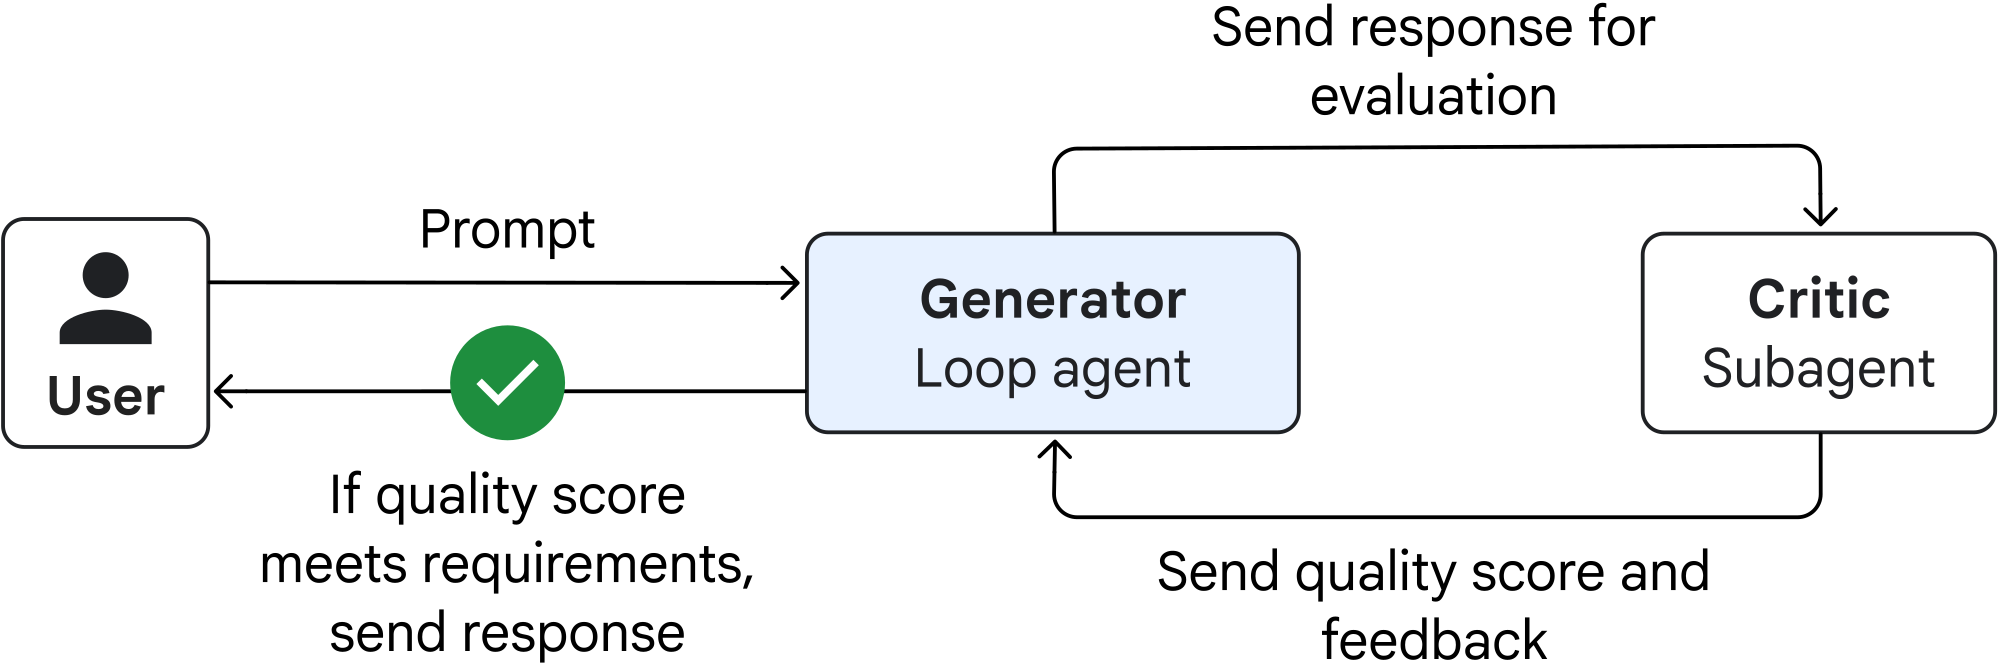
\includegraphics[width=\linewidth]{figures/deck/gcp-review-and-critique.png}
    \caption{Review and critique}
    \label{fig:patterns-review}
  \end{subfigure}\hfill
  \begin{subfigure}[b]{0.48\textwidth}
    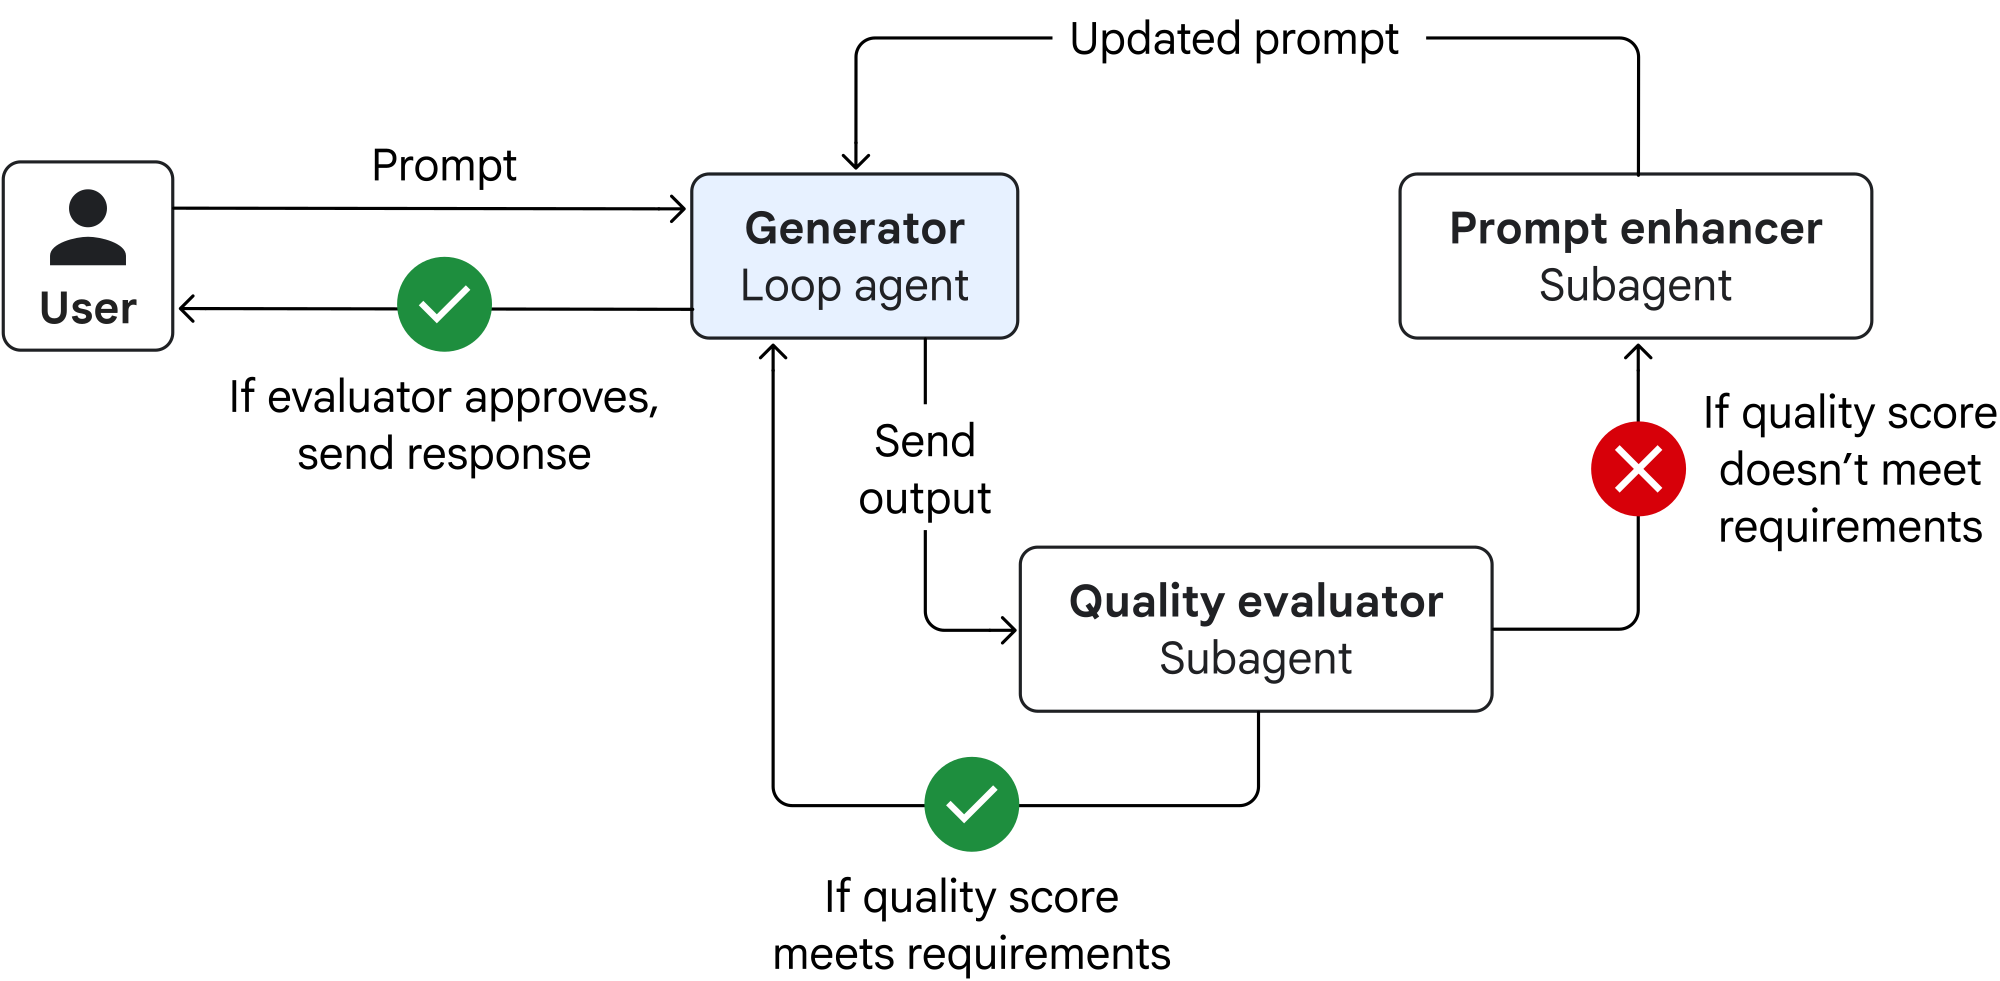
\includegraphics[width=\linewidth]{figures/deck/gcp-iterative-refinement.png}
    \caption{Iterative refinement}
    \label{fig:patterns-refinement}
  \end{subfigure}
  \caption{Patterns orchestrated by a model inside one agent (a) and by predefined logic (b to f).
  The review and critique pattern (e) and the iterative refinement pattern (f) are loops run by
  predefined logic. Google Cloud Architecture Center, agentic design patterns, CC BY 4.0.}
  \label{fig:patterns-react-to-refinement}
\end{figure*}

\subsection{Reason and act}
\label{sec:patterns-react}

In the \textbf{reason and act} pattern, one agent repeats a cycle of thought, action and
observation (\cref{fig:patterns-react}). The pattern is the reactive loop of \cref{sec:reactive},
and the model decides every next step.

In the thought, the model reasons about what to do next. In the action, it calls a tool. In the
observation, it reads the tool's result. The cycle repeats until the model gives an answer, the run
reaches a cap on the number of iterations, or an error stops it. The cap plays the role of the
budget, the limit on model calls that stops a reactive loop (\cref{sec:reactive-stops}).
\bi
\item \textbf{Who orchestrates.} The model orchestrates, inside one agent. No other component
chooses the next tool call. The model chooses it after reading the previous observation.
\item \textbf{When to use it.} We use reason and act when the task is dynamic, meaning that the
right next step depends on what the last step returned. In our running example, whether \msa{}
should read a helper function in another file depends on what its first read of the flagged code
showed (\cref{sec:fixed-costs}).
\item \textbf{When it is a poor choice.} Reason and act is a poor choice when a single query to the
model would answer the user's request, the prompt that starts the run. Every cycle adds a model
call, so the pattern's \textbf{latency}, the time the user waits for the response, is higher than
that of a single call. Every observation also feeds the next decision, so a misleading tool result
can carry through to the final answer.
\ei

\subsection{Sequential, parallel and loop}
\label{sec:patterns-predefined}

In the sequential, parallel and loop patterns, predefined logic orchestrates. The program decides in
advance which subagents run, how they are arranged, and what ends the work.

In the \textbf{sequential} pattern, specialists run one after another in a fixed linear order, and
the output of each one is the input of the next (\cref{fig:patterns-sequential}).
\bi
\item \textbf{Who orchestrates.} Predefined logic orchestrates. The order is written into the
program before the run, so the agents run in a fixed order, as the steps of a fixed workflow do.
\item \textbf{When to use it.} The pattern suits a process in which every input needs the same steps
in the same order, for example extracting data, then cleaning it, then loading it.
\item \textbf{When it is a poor choice.} The sequential pattern is a poor choice when some runs do
not need every step. The fixed order makes every run execute all of them, so a slow step that a run
did not need still delays its response.
\ei

In the \textbf{parallel} pattern, independent workers carry out separate parts of the task at the
same time (\cref{fig:patterns-parallel}). A \textbf{gather step}, also called the join, then
combines their results into one response.
\bi
\item \textbf{Who orchestrates.} Predefined logic orchestrates. It decides which workers run and
that the gather step receives all of their results.
\item \textbf{When to use it.} We use the parallel pattern when the work splits into parts that do
not depend on one another's results, for example collecting information from several sources at
once.
\item \textbf{When it is a poor choice.} The parallel pattern is a poor choice when the workers'
results can conflict. The workers do not read one another's records, so nothing keeps their results
consistent. The gather step must then decide which result to keep, or how to merge them, before it
can produce one response. Every worker also makes its own model calls, so cost and token use grow
with the number of workers.
\ei

In the \textbf{loop} pattern, a sequence of subagents runs repeatedly until an exit condition holds
(\cref{fig:patterns-loop}). An \textbf{exit condition} is a test that ends the loop when it is
satisfied, such as a maximum number of iterations or a required state. It is usually checked after
each pass, although the designer can place the check at any point in the sequence. The loop pattern differs from reason and act in who chooses the
steps. In the loop pattern, the sequence of subagents is the same on every pass. In reason and act,
the model chooses each next step.
\bi
\item \textbf{Who orchestrates.} Predefined logic orchestrates, because both the sequence and the
exit condition are written before the run.
\item \textbf{When to use it.} We use the loop pattern when the work needs repeated passes, or needs
to correct its own earlier output, before it is good enough.
\item \textbf{When it is a poor choice.} The loop pattern is a poor choice when its exit condition
is not clearly defined. A loop whose exit condition never holds keeps running until its budget, the
limit on model calls, stops it. A budget guarantees that the loop stops. It does not guarantee that
the work is finished (\cref{sec:fixed-guarantees}).
\ei

\subsection{Loops of generation and evaluation}
\label{sec:patterns-review}

The review and critique pattern and the iterative refinement pattern are both loops run by
predefined logic. In each of them, one component produces a result and another evaluates it.

In the \textbf{review and critique} pattern, a \textbf{generator} produces a \textbf{candidate}, an
output proposed for acceptance, and a \textbf{critic} judges it against stated criteria
(\cref{fig:patterns-review}). The critic approves the candidate, rejects it, or returns a quality
score with feedback, which the generator uses to revise. When a candidate meets the criteria, the
generator returns it as the response. The generator proposes and the critic accepts, which is the
separation that the validator makes for the patches of \msa{} (\cref{sec:validation}).
\bi
\item \textbf{Who orchestrates.} Predefined logic runs the pattern as a loop. The program sends
every candidate to the critic and repeats the cycle until the critic approves.
\item \textbf{When to use it.} We use review and critique when the output has to be accurate or has
to meet strict rules, for example code that must pass an audit.
\item \textbf{When it is a poor choice.} Review and critique is a poor choice when speed matters.
Every evaluation is at least one more model call, and each revision the critic asks for adds a new
candidate and a new evaluation.
\ei

In the \textbf{iterative refinement} pattern, one or more agents improve a result held in state over
repeated cycles (\cref{fig:patterns-refinement}). The cycles stop when the result reaches a
\textbf{quality threshold}, a minimum score set in advance, or when the number of cycles reaches a
cap. In the diagram, the generator's output goes to a quality evaluator. If the score meets the
threshold, the generator returns the result. If it does not, a prompt enhancer, a subagent that
rewrites the generator's prompt, produces a new prompt, and the generator tries again.
\bi
\item \textbf{Who orchestrates.} Predefined logic runs the loop, as in review and critique.
\item \textbf{When to use it.} We use iterative refinement when the task is hard to get right in one
pass, for example drafting a document or debugging.
\item \textbf{When it is a poor choice.} Iterative refinement is a poor choice when the exit
condition is vague, for example a quality threshold that is never stated precisely. Each cycle
costs time and money whether or not it improves the result.
\ei

The two patterns differ in what the loop is for. In review and critique, the loop decides whether
to accept a candidate. In iterative refinement, the loop improves one result from cycle to cycle.

\begin{figure*}[t]
  \centering
  % Coordinator, hierarchical and human in the loop stack on the left; the swarm takes the right.
  % The counter is set by hand so the letters follow the slides: (c) swarm, (d) human in the loop.
  \begin{minipage}[c]{0.6\textwidth}
    \centering
    \begin{subfigure}[b]{0.45\linewidth}
      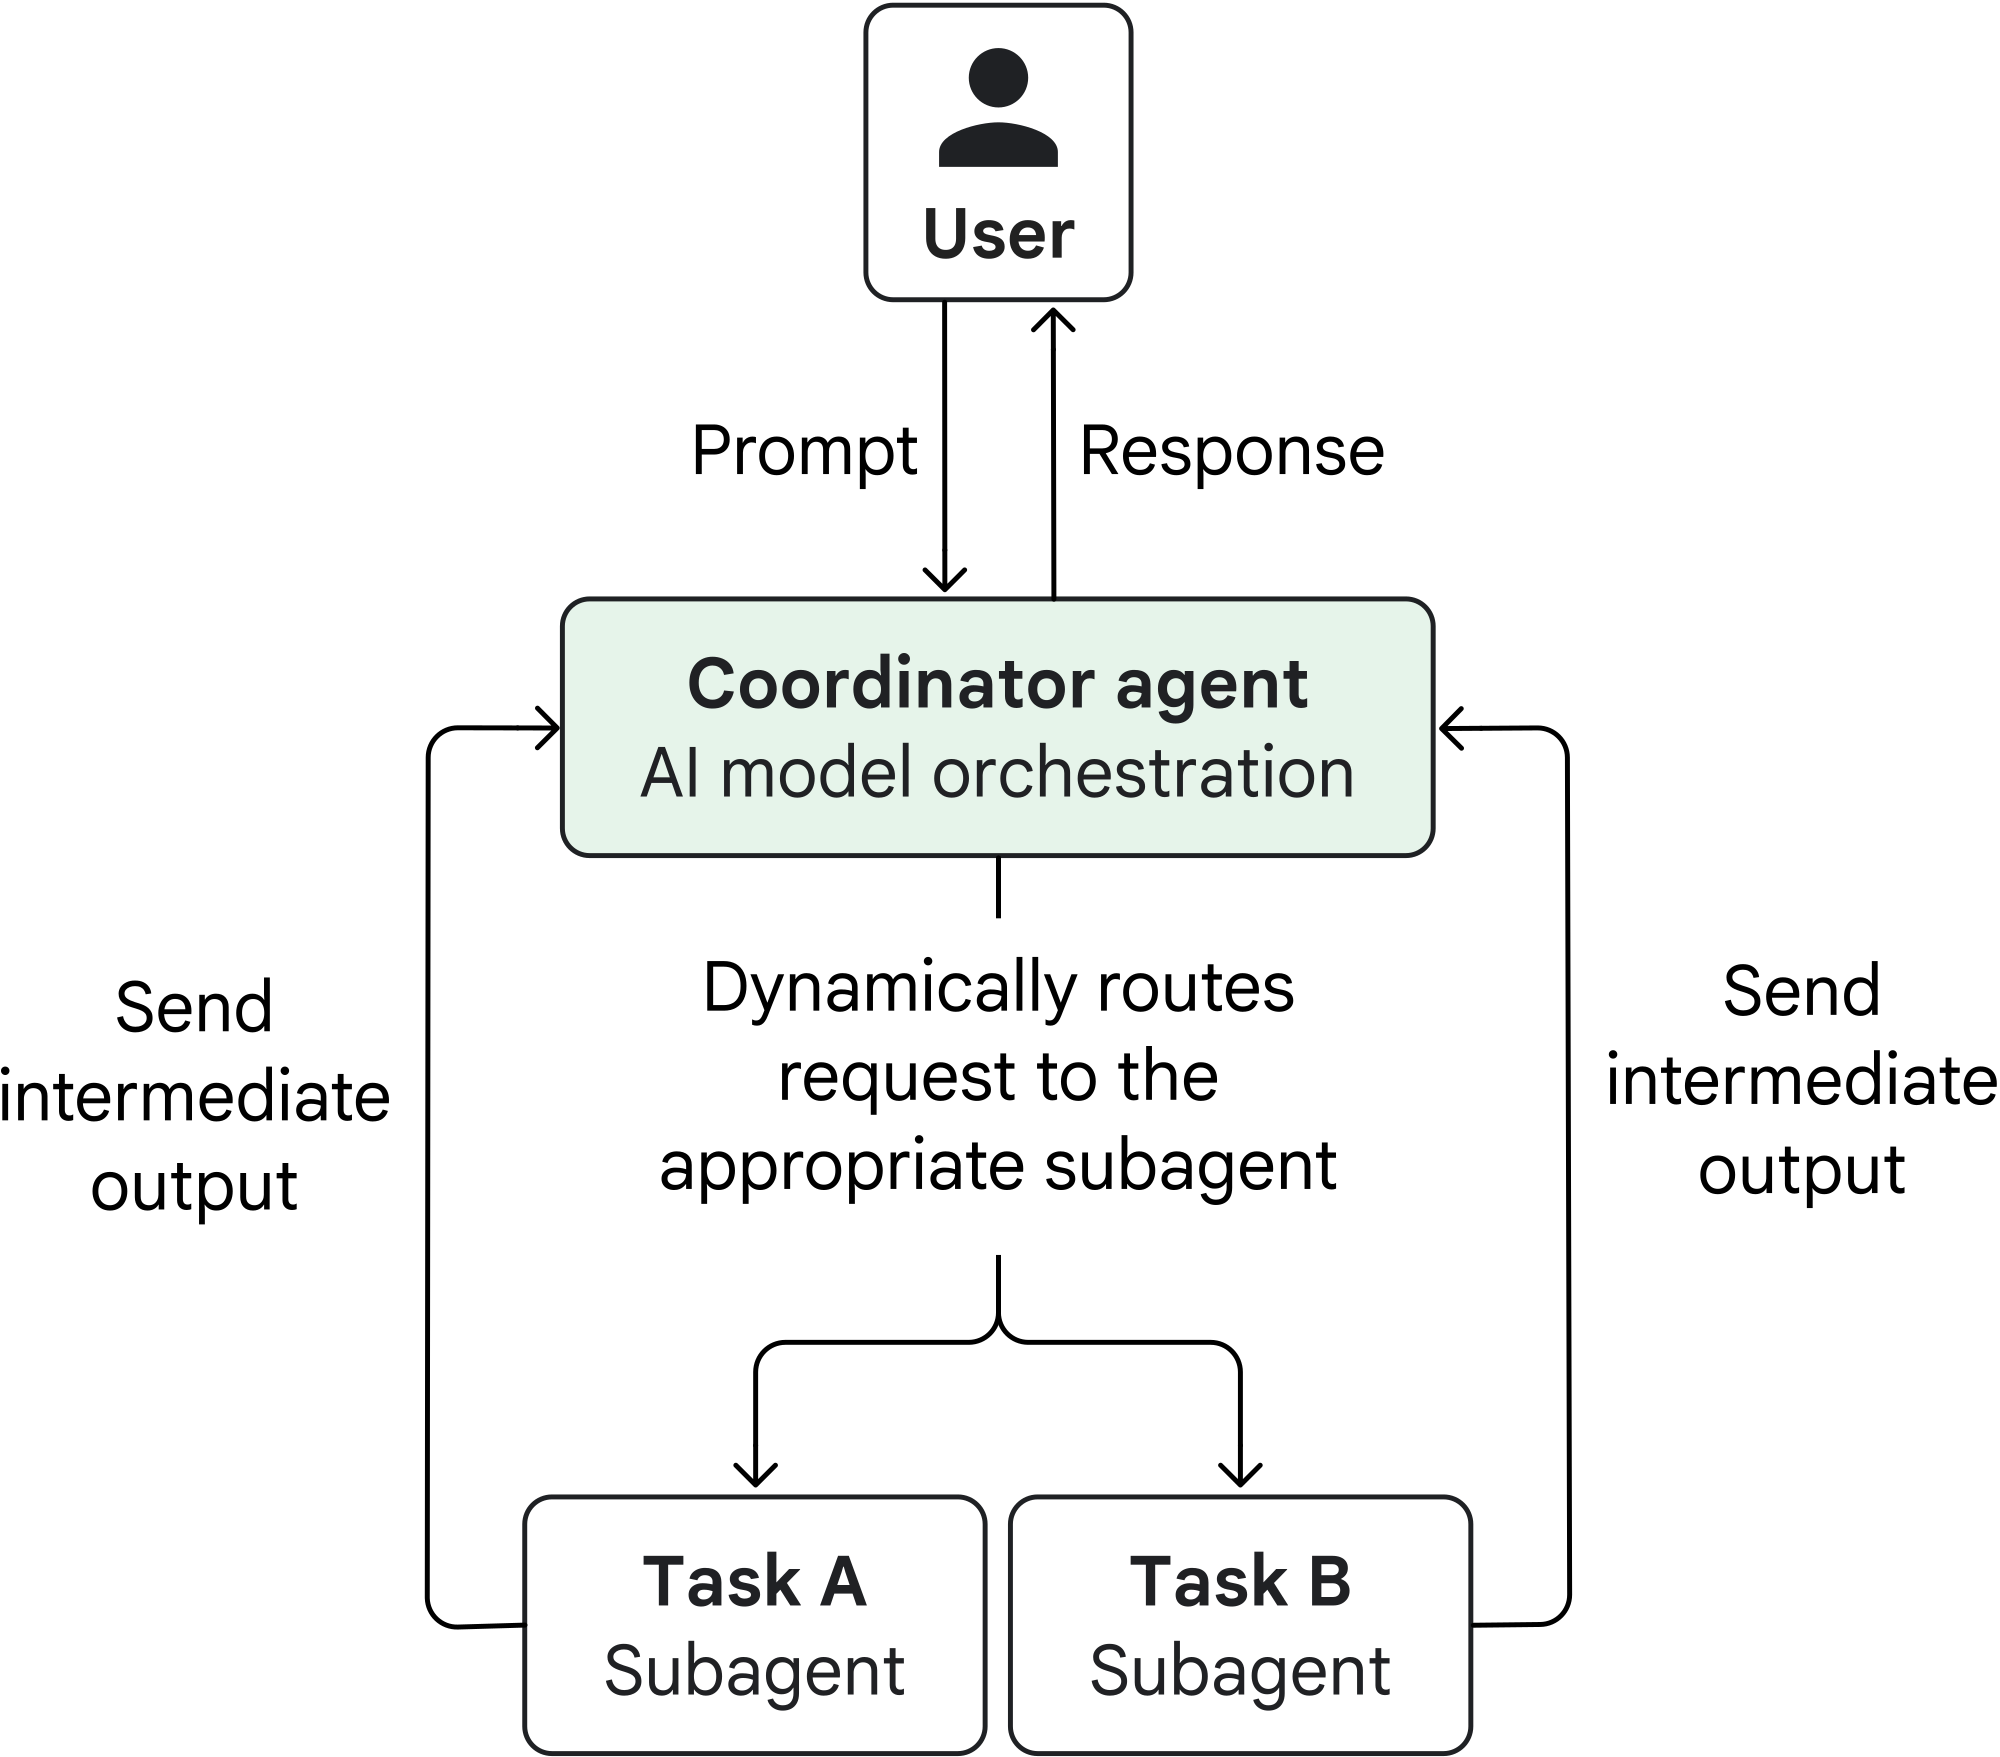
\includegraphics[width=\linewidth]{figures/deck/gcp-coordinator.png}
      \caption{Coordinator}
      \label{fig:patterns-coordinator}
    \end{subfigure}\hfill
    \begin{subfigure}[b]{0.52\linewidth}
      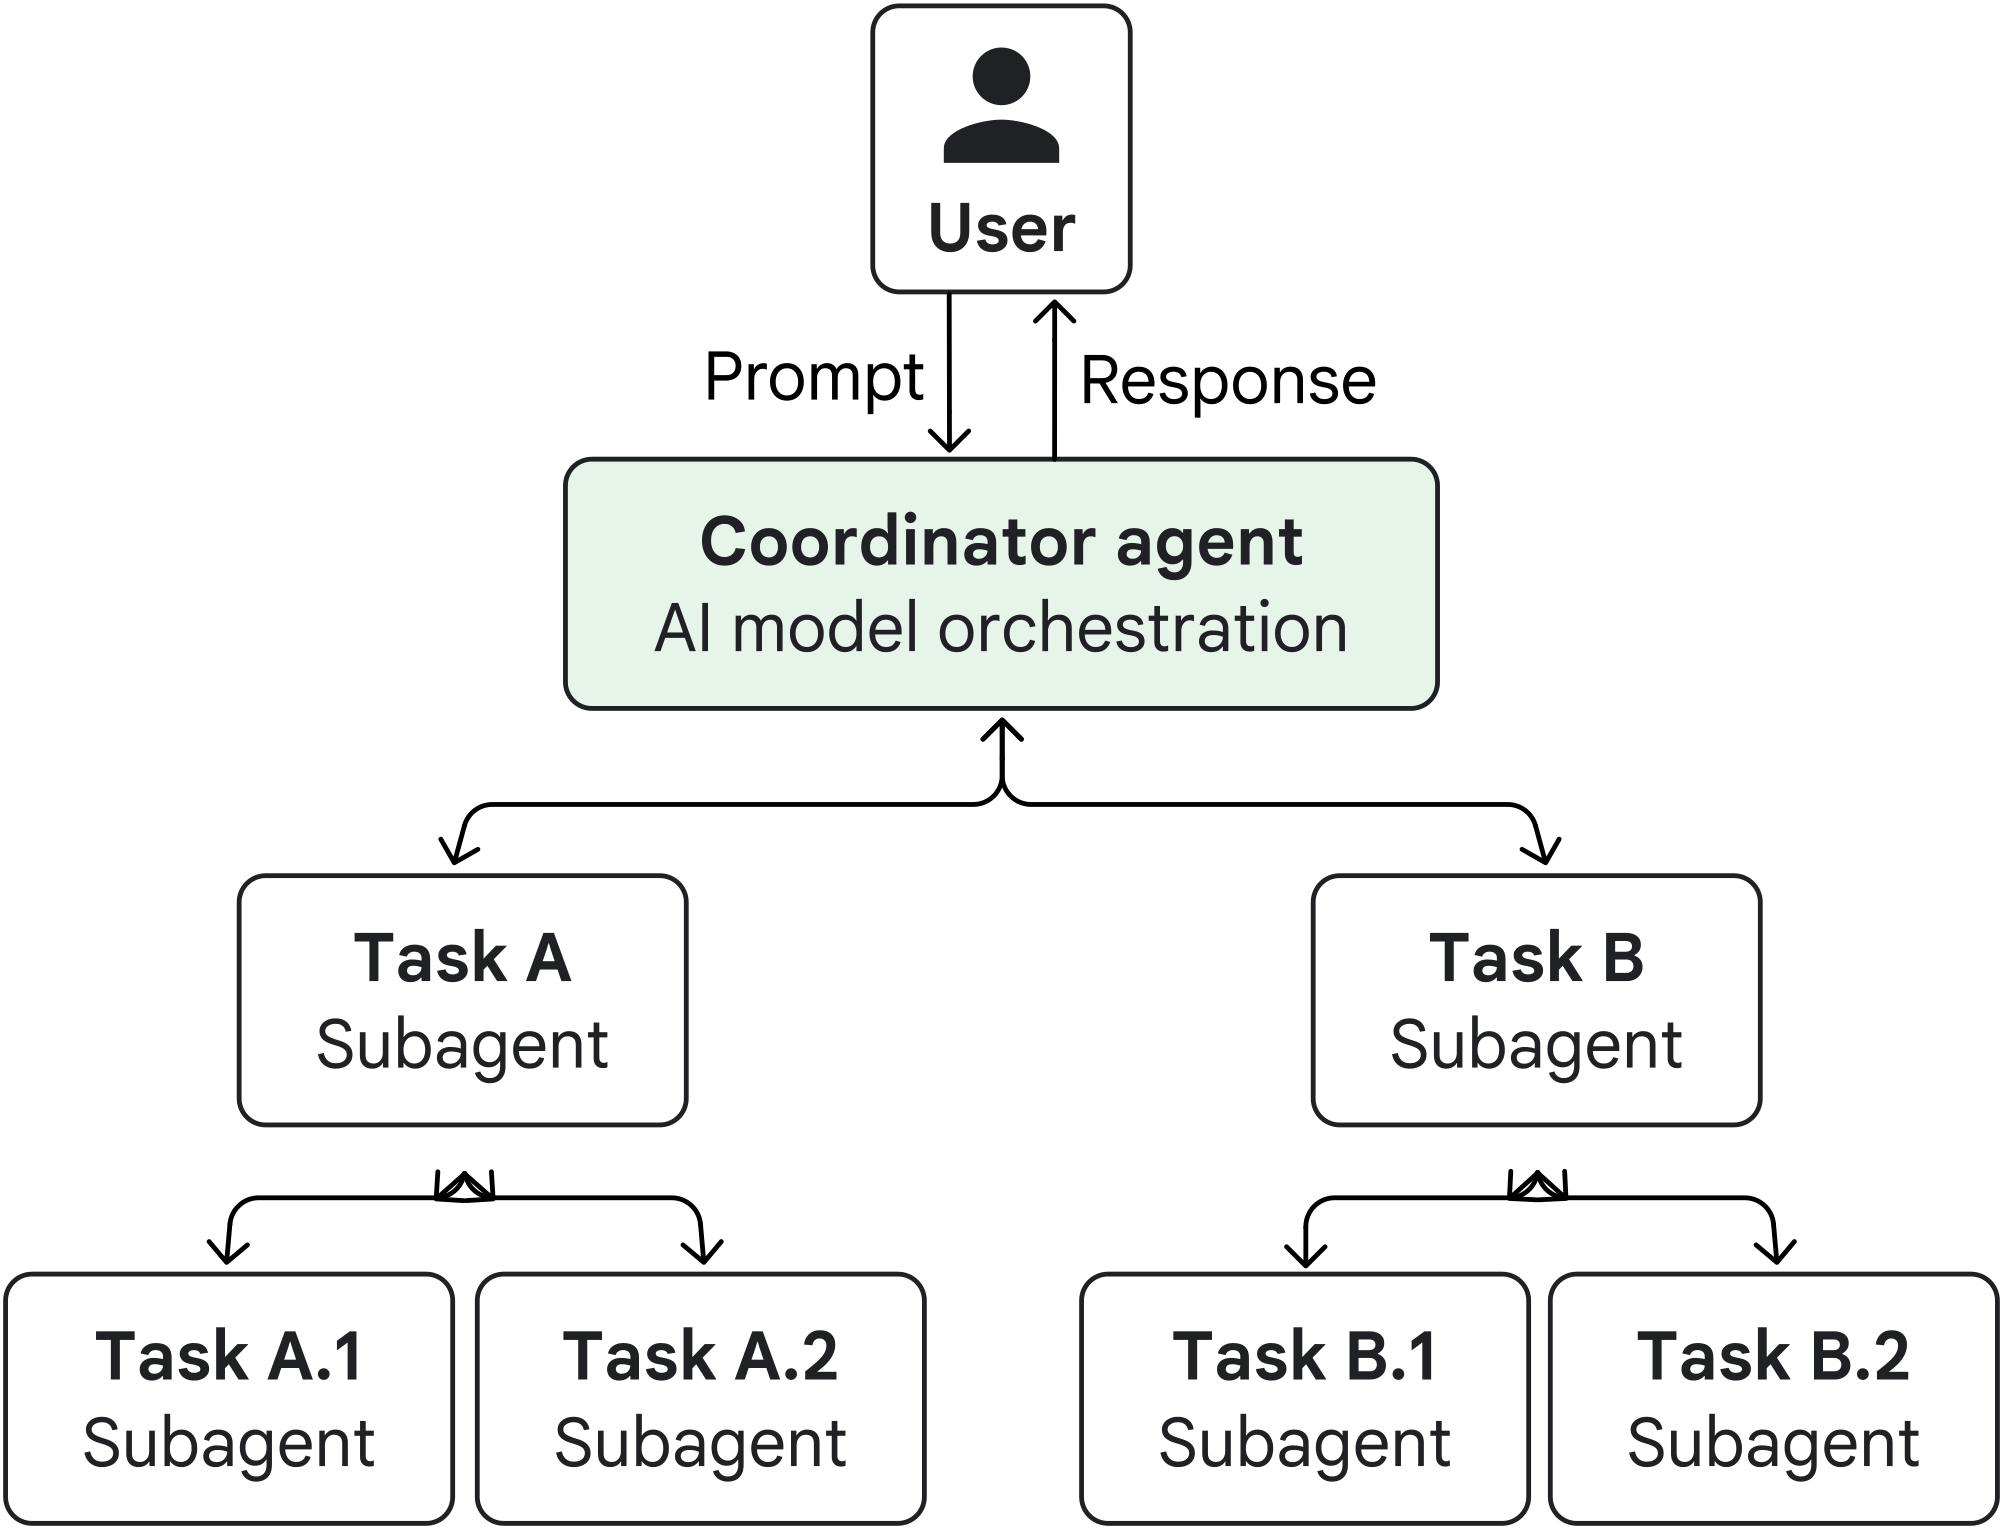
\includegraphics[width=\linewidth]{figures/deck/gcp-hierarchical-task-decomposition.png}
      \caption{Hierarchical task decomposition}
      \label{fig:patterns-hierarchical}
    \end{subfigure}

    \medskip
    \setcounter{subfigure}{3}%
    \begin{subfigure}[b]{\linewidth}
      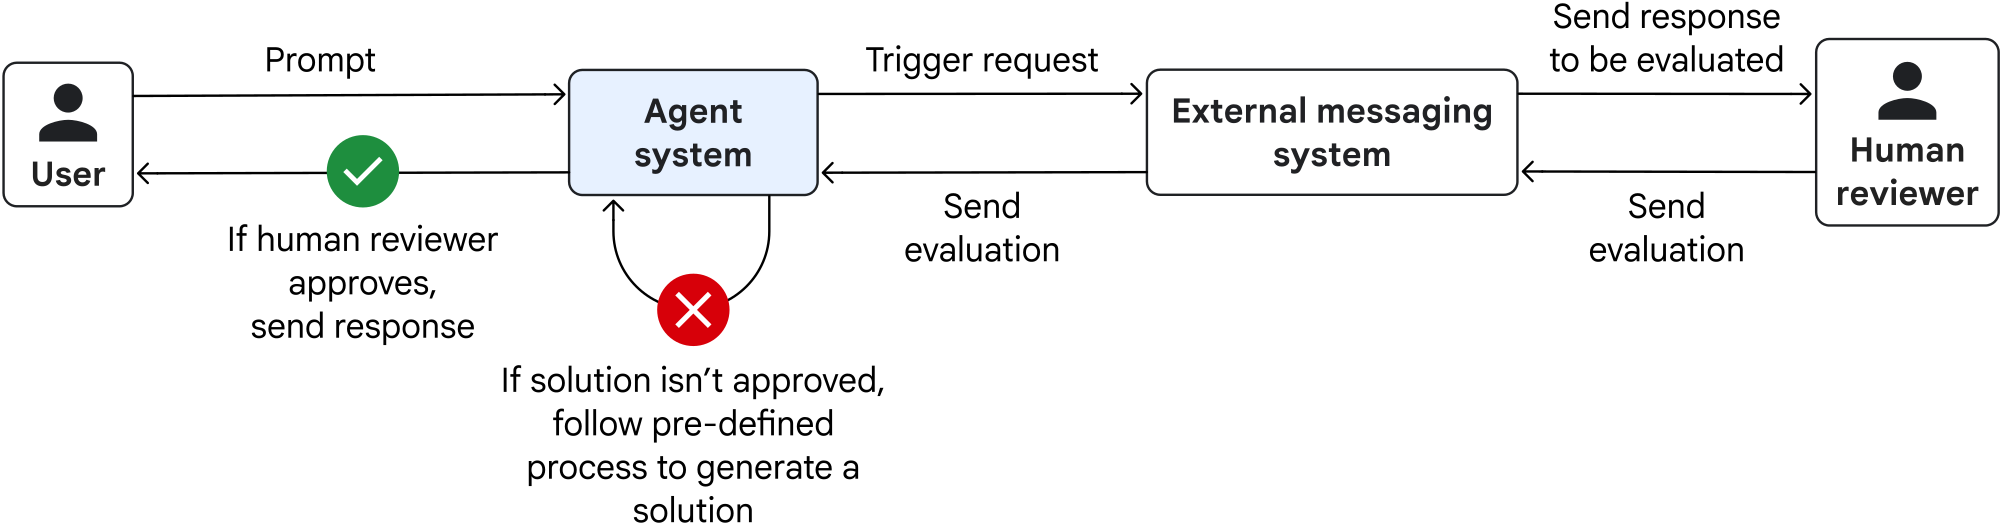
\includegraphics[width=\linewidth]{figures/deck/gcp-human-in-the-loop.png}
      \caption{Human in the loop}
      \label{fig:patterns-hitl}
    \end{subfigure}
  \end{minipage}\hfill
  \begin{minipage}[c]{0.38\textwidth}
    \setcounter{subfigure}{2}%
    \begin{subfigure}[b]{\linewidth}
      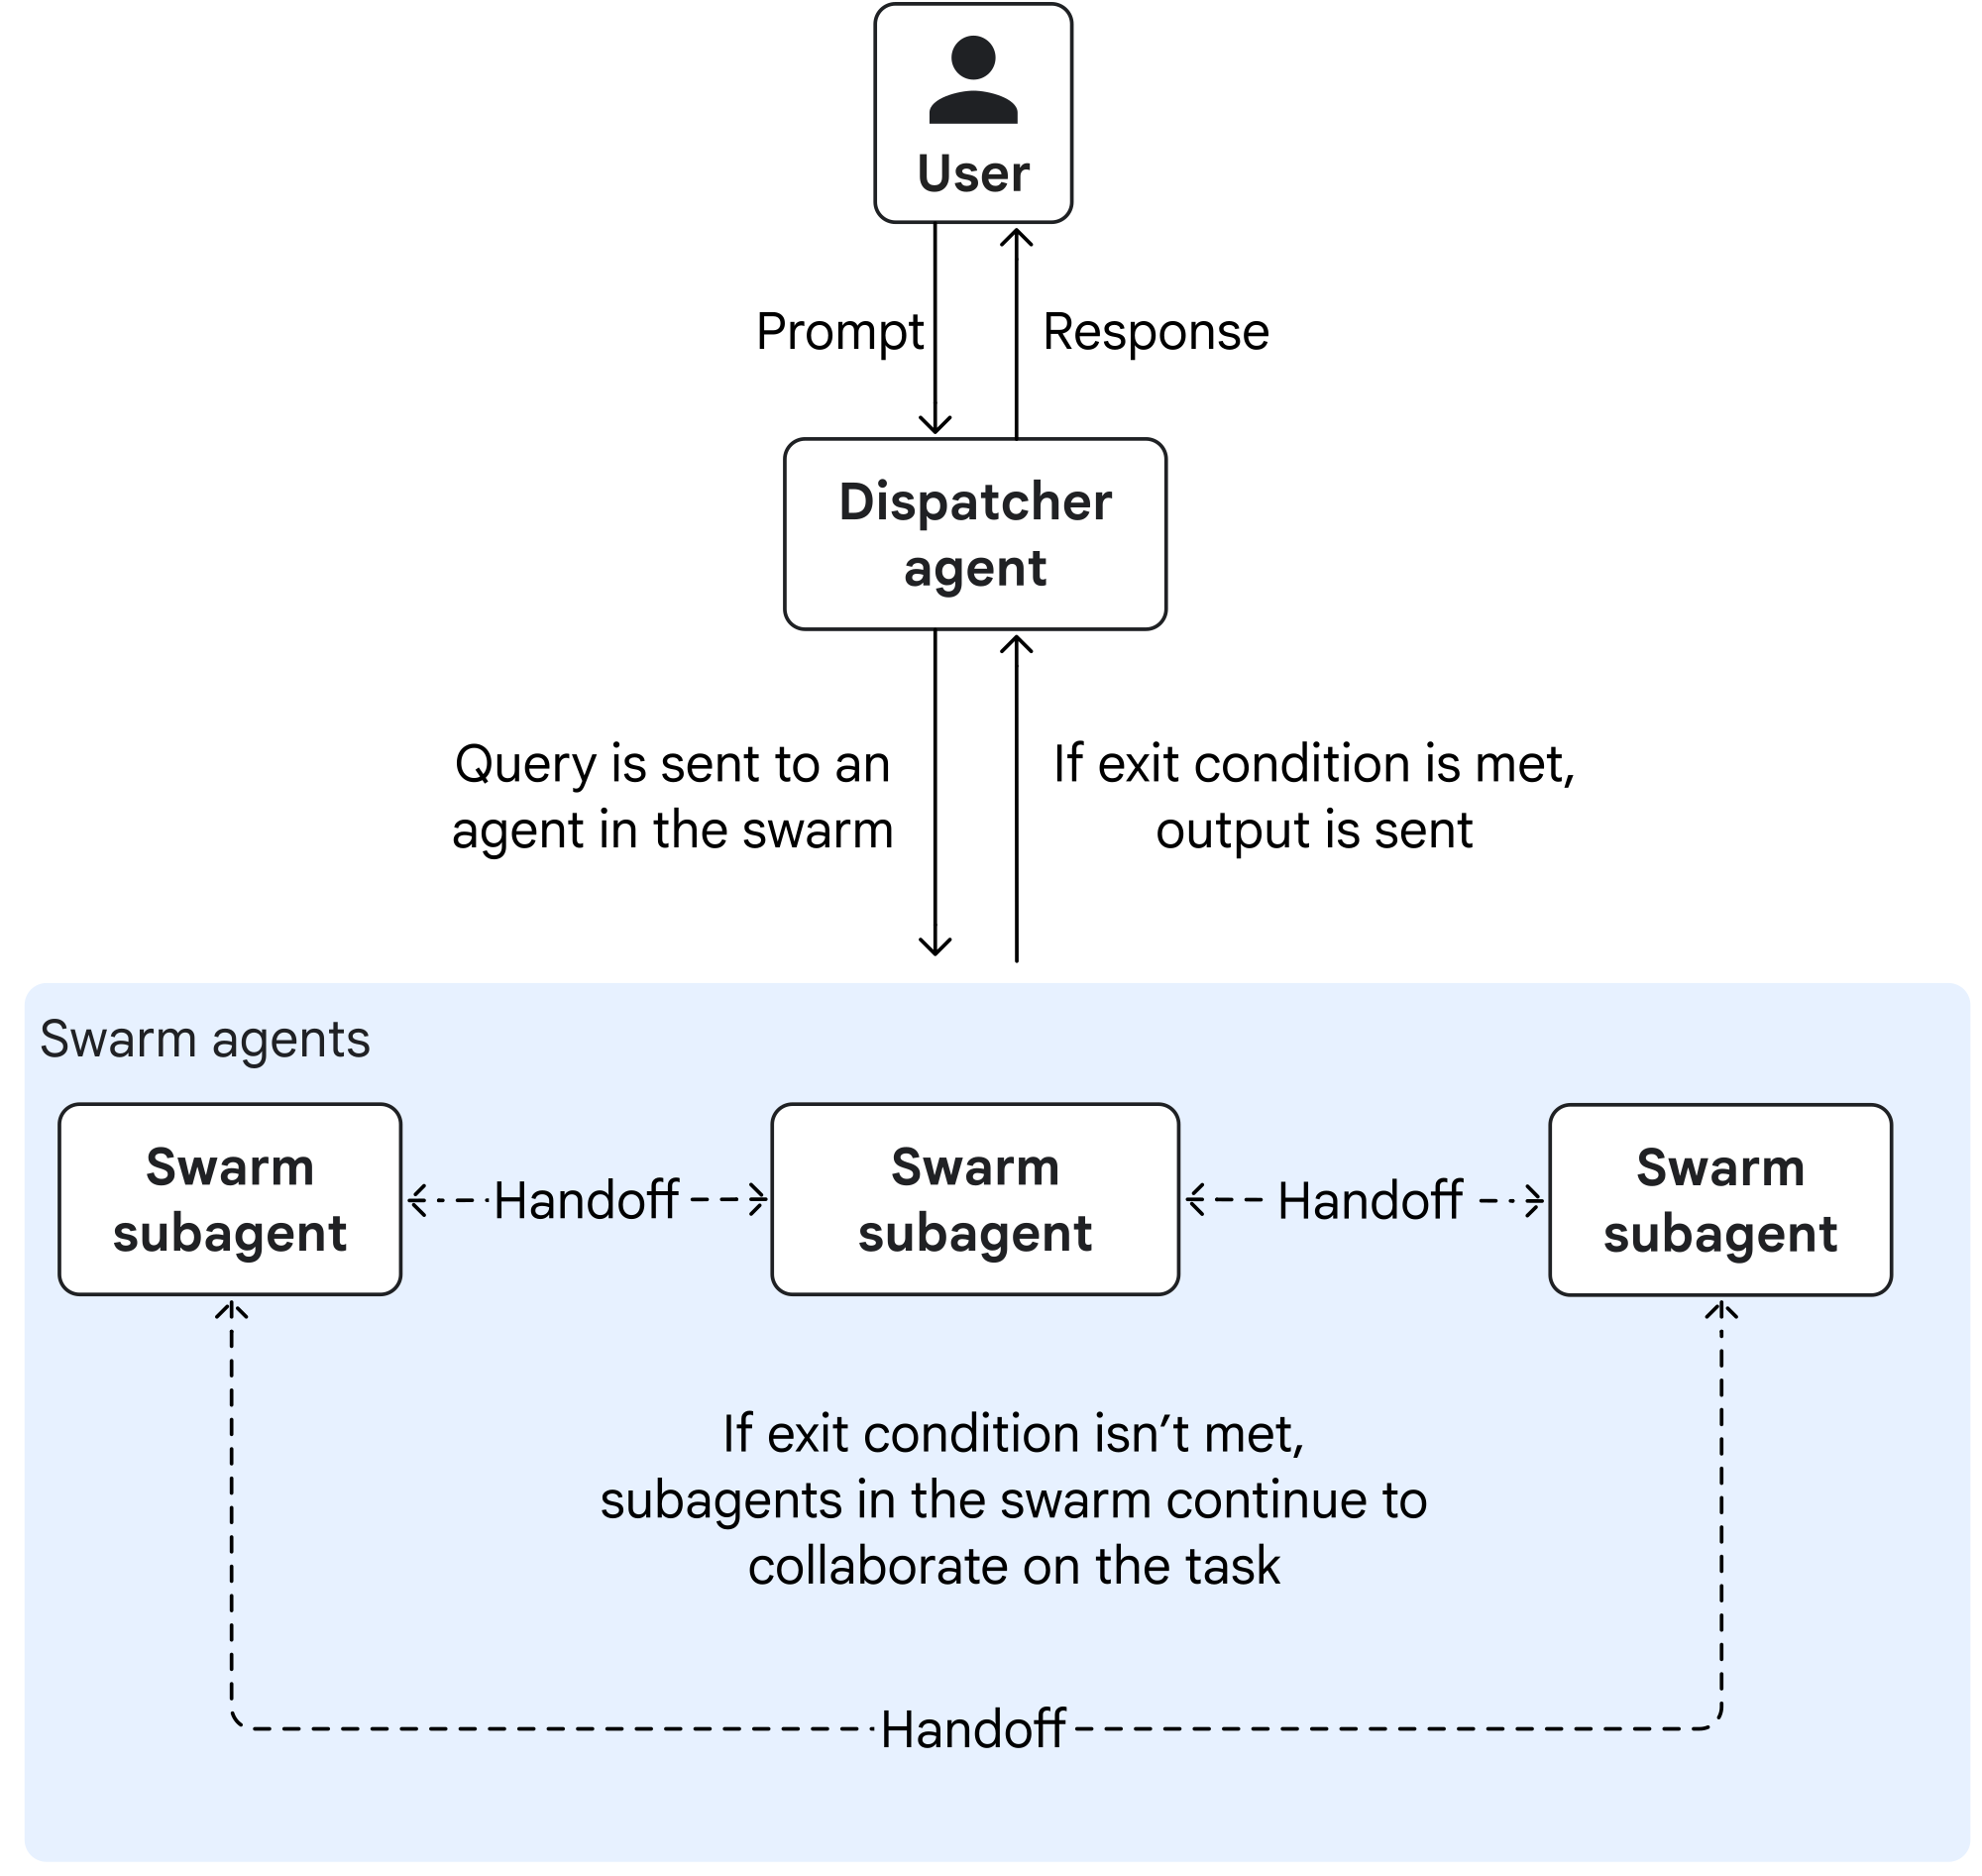
\includegraphics[width=\linewidth]{figures/deck/gcp-swarm.png}
      \caption{Swarm}
      \label{fig:patterns-swarm}
    \end{subfigure}
  \end{minipage}
  \caption{Patterns orchestrated by a model (a, b), with no central orchestrator (c), and by
  predefined checkpoints (d). Google Cloud Architecture Center, agentic design patterns, CC BY 4.0.}
  \label{fig:patterns-coordinator-to-hitl}
\end{figure*}

\subsection{Coordinator and hierarchical task decomposition}
\label{sec:patterns-coordinator}

In the coordinator pattern and the hierarchical task decomposition pattern, a model orchestrates
other agents. It decides at run time how the task is divided and which agent does each part.

\Cref{fig:patterns-coordinator-to-hitl} shows the coordinator, hierarchical task decomposition,
swarm and human-in-the-loop patterns as the catalogue draws them. The catalogue draws custom logic
only through one example, a refund process that runs a parallel check and then a conditional
branch. We do not reproduce that example, because custom logic has no general shape: its shape is
whatever conditional code the team writes.

In the \textbf{coordinator} pattern, a central agent reads the request, splits it into parts, and
sends each part to a specialist (\cref{fig:patterns-coordinator}). The choice of which specialist
receives each part is the coordinator's routing decision. The specialists send their results back
to the coordinator, which assembles the response.
\bi
\item \textbf{Who orchestrates.} A model orchestrates. The coordinator uses a model to make the
routing decision, so the routing is decided at run time from the content of the request.
\item \textbf{When to use it.} We use the coordinator pattern when the routing must adapt to the
request. This is the case when we can tell which specialists a request needs only after reading it.
\item \textbf{When it is a poor choice.} The coordinator pattern is a poor choice when a single agent
could do the work, because the coordinator adds model calls, tokens and latency to every request.
\ei

In the \textbf{hierarchical task decomposition} pattern, a root agent splits the task into
subtasks, and each subagent may split its subtask again (\cref{fig:patterns-hierarchical}).
Splitting continues until each piece is small enough for a worker to carry out directly. The result
is a tree of agents, with the root at the top and the workers at the leaves.
\bi
\item \textbf{Who orchestrates.} A model orchestrates at several levels, because every split is a
model's decision. Every agent that splits its task plays the coordinator's role for the agents
below it. In the diagram, the root agent is labeled a coordinator agent.
\item \textbf{When to use it.} We use hierarchical task decomposition when the problem is
open-ended and needs research, planning and synthesis together. A problem is open-ended when its
subtasks cannot be listed in advance, and synthesis is the combining of findings into one answer.
\item \textbf{When it is a poor choice.} Hierarchical task decomposition is a poor choice when the
system has to be easy to debug. The tree has many agents and many model calls, so finding the
decision that caused a wrong result is hard.
\ei

\subsection{Swarm, human in the loop, and custom logic}
\label{sec:patterns-other}

The swarm, the human-in-the-loop pattern and custom logic each give a different answer to the
question of who orchestrates. A swarm has no central orchestrator. The human-in-the-loop pattern is
orchestrated by predefined checkpoints, and custom logic by code the team writes.

In a \textbf{swarm}, several specialists communicate with one another directly and refine a result
together until an explicit exit condition is met (\cref{fig:patterns-swarm}). Any specialist can
pass the work to any other. A \textbf{handoff} is one such transfer of the work from one agent to
another.

In the diagram, an entry agent labeled the dispatcher agent passes the request into the swarm. It
returns the output once the exit condition is met. It does not direct the work inside the swarm.
This agent is unrelated to the dispatcher that Lecture~4 studies, the runtime component that
executes tool calls.
\bi
\item \textbf{Who orchestrates.} No central component orchestrates. Each agent chooses for itself
when to hand off and to whom, so no single component decides which agent acts next.
\item \textbf{When to use it.} We use a swarm when the problem is ambiguous, that is, when it has no
single agreed framing, and it benefits from argument between different perspectives.
\item \textbf{When it is a poor choice.} In most other cases a swarm is a poor choice. Every handoff
adds model calls, and the exchanges continue until the exit condition is met. The catalogue
therefore describes the swarm as the most complex and costly multi-agent pattern to implement. A
swarm may also never \textbf{converge}, which
means that the agents may never reach a result that satisfies the exit condition.
\ei

In the \textbf{human-in-the-loop} pattern, the agent pauses at a checkpoint and waits for a person to
approve its work, correct it, or supply missing input (\cref{fig:patterns-hitl}). In the diagram,
the agent sends its result through an external messaging system to a human reviewer. If the
reviewer approves, the agent returns the response. If not, the agent follows a predefined process
to produce a new solution.
\bi
\item \textbf{Who orchestrates.} Predefined checkpoints orchestrate this pattern, because the points
where the run stops for a person are fixed at design time.
\item \textbf{When to use it.} We use the human-in-the-loop pattern when the decision is high-stakes
or subjective, for example a payment or a sensitive document.
\item \textbf{When it is a poor choice.} The human-in-the-loop pattern is a poor choice when no
person is available to answer. The pattern also requires an interaction system, such as the
messaging system in the diagram, that has to be built and then maintained.
\ei

In the \textbf{custom logic} pattern, the orchestration is conditional code that the team building
the system writes, combining the other patterns as the task requires.

Custom logic is written before the run, as predefined logic is. The difference lies in the shape of
the code. Predefined logic follows one of the fixed structures of the named patterns: a sequence, a
set of workers whose results are gathered, or a loop. Custom logic can branch in any way the team
chooses.
\bi
\item \textbf{Who orchestrates.} Code that the team writes orchestrates. The team writes every
branch and the condition that selects it, although a condition may test a value that the model
produced.
\item \textbf{When to use it.} We use custom logic when the branching goes beyond a linear sequence,
or when fixed rules have to be mixed with model reasoning.
\item \textbf{When it is a poor choice.} Custom logic is a poor choice when one of the named patterns
already matches the task. The team would then own the whole flow and have to debug all of it.
\ei

\subsection{Axes for comparing patterns}
\label{sec:patterns-axes}

\begin{table*}[t]
  \caption{The axes of comparison applied to patterns that a model orchestrates (coordinator,
  hierarchical task decomposition) and to patterns that predefined logic orchestrates (parallel,
  review and critique).}
  \label{tab:patterns-axes}
  \begin{adjustbox}{width=\linewidth}\begin{tabularx}{\linewidth}{L{0.175\linewidth}XXXX}
    \toprule
    \textbf{Axis} & \textbf{Coordinator} & \textbf{Hierarchical task decomposition} &
      \textbf{Parallel} & \textbf{Review and critique} \\
    \midrule
    \textbf{Task ownership} & The coordinator owns the task and delegates pieces. Each specialist
      owns only its piece.
      & Nested. Each level owns the decomposition it made.
      & Each worker owns one independent piece. The gather step owns the whole.
      & The generator owns the candidate. The critic owns acceptance. \\ \addlinespace
    \textbf{State boundaries} & Separate contexts. Only what the coordinator passes crosses.
      & One boundary per level. Partial results cross upward.
      & One state record per worker. The gather step reads all of them.
      & No new boundary. One shared record, with the critic's reasons added. \\ \addlinespace
    \textbf{Model-call}\newline\textbf{overhead} & One routing call per request, plus the
      specialists' calls.
      & Multiplied by the depth of the hierarchy.
      & The sum of the workers' calls, made concurrently.
      & One critic call per candidate, plus one generator call per revision. \\ \addlinespace
    \textbf{Latency} & The routing call is on the critical path.
      & Each level adds a round trip.
      & Reduced to the slowest worker plus the gather step.
      & Each revision adds a round trip. \\ \addlinespace
    \textbf{Failure propagation} & A misrouted task fails inside the wrong specialist, and the
      coordinator may not notice.
      & A wrong decomposition spreads downward, and its cost multiplies.
      & Contained in each worker until the gather step, where a missing piece blocks the whole.
      & A wrong acceptance passes the candidate on. A wrong rejection costs a revision. \\ \addlinespace
    \textbf{Inspectability} & The routing decision and its reasons are in the trace, if recorded.
      & Traces nest. The trace must record which level made each decision.
      & Traces interleave. The trace must record which worker wrote each event.
      & Better than when the generator accepts its own output. Each acceptance carries the critic's
      reasons. \\
    \bottomrule
  \end{tabularx}\end{adjustbox}
\end{table*}

Several patterns can often perform the same task. Choosing among them requires comparing what each
one costs and what each one lets us see. We make the comparison along \textbf{axes}, each a
property of a pattern that can be examined across patterns. We apply the axes to patterns of both
kinds. A model orchestrates the coordinator pattern and hierarchical task decomposition. Predefined
logic orchestrates the parallel pattern and the review and critique pattern. Comparing patterns of
both kinds shows how the choice between a model and predefined logic affects each axis.

Each axis asks one question about a pattern:
\bi
\item \textbf{Task ownership.} Which component is responsible for the whole task, and which only
for a piece of it?
\item \textbf{State boundaries.} What can each component see, and what information has to cross
from one component to another?
\item \textbf{Model-call overhead.} How many model calls does the pattern's structure add, and how
many calls does a request then cost in total?
\item \textbf{Latency.} How much longer does the user wait for the response to a single request
because of the pattern's structure? The answer depends on the \textbf{critical path}, the longest
sequence of steps that must happen one after another before the response is ready, and on each
\textbf{round trip}, the time taken to send work to a component and receive its result.
\item \textbf{Failure propagation.} Where does a mistake go after it is made, and which component
can notice it?
\item \textbf{Inspectability.} What can a person reading the trace after the run reconstruct about
which component decided what?
\ei

\Cref{tab:patterns-axes} summarizes the comparison. Each row is one axis, and reading a row across
the columns shows how the patterns differ on that axis. The columns for the coordinator and for
hierarchical task decomposition hold the patterns that a model orchestrates. Comparing them with the
other two columns shows where a control decision made at run time adds cost or risk.

\subsection{Task ownership and state boundaries}
\label{sec:patterns-ownership}

Task ownership and state boundaries describe how a pattern divides responsibility and information
among its components. Task ownership says which component is responsible for each part of the
result. State boundaries say what each component can see.

Task ownership differs across the patterns as follows:
\bi
\item \textbf{Coordinator.} The coordinator owns the whole task and delegates pieces of it. Each
specialist owns only the piece it received.
\item \textbf{Hierarchical task decomposition.} Ownership is nested. Each level owns the
decomposition it made, and the workers at the leaves own only the pieces they carry out.
\item \textbf{Parallel.} Each worker owns one independent piece. The gather step owns the whole,
because it is the only component that receives every result.
\item \textbf{Review and critique.} The generator owns the candidate, and the critic owns the
decision to accept it.
\ei

A run's state is the record of the run so far, which its components read and write, and a model's
context is the input it receives in one call (\cref{sec:reactive-loop}). A \textbf{state boundary} determines which parts of the state reach which model's context. It differs
across the patterns as follows:
\bi
\item \textbf{Coordinator.} The coordinator's context and each specialist's context are separate.
Only what the coordinator passes to a specialist crosses, so a specialist works from the
coordinator's description of its piece.
\item \textbf{Hierarchical task decomposition.} There is a state boundary at every level. Partial
results cross upward, from the workers to the agent that split their task, and from there toward
the root.
\item \textbf{Parallel.} Each worker keeps its own state record, and the gather step reads all of
them. The workers do not read one another's records, which keeps them independent.
\item \textbf{Review and critique.} The pattern adds no state boundary. The generator and the
critic work on one record, as a single agent would, and the critic adds its reasons to it.
\ei

\subsection{Model-call overhead and latency}
\label{sec:patterns-cost}

Model-call overhead and latency measure what a pattern costs. Model-call overhead counts the model
calls that the pattern's structure adds, such as the coordinator's routing call, and the total that
a request then costs. Latency measures how much longer the user waits for the response to a single
request.

A request can be no faster than its critical path. The patterns compare as follows:
\bi
\item \textbf{Coordinator.} The overhead is one routing call per request, plus the specialists'
calls. The routing call is on the critical path, because no specialist can start until the
coordinator has decided where the request goes.
\item \textbf{Hierarchical task decomposition.} The overhead is multiplied by the depth of the
hierarchy, its number of levels, because every level that splits a task makes calls of its own.
Each level also adds a round trip, because a level waits for the results of the level below it.
\item \textbf{Parallel.} The overhead is the sum of the workers' calls, which are made
concurrently. The latency falls to that of the slowest worker plus the gather step, because the
workers run at the same time.
\item \textbf{Review and critique.} The overhead is one critic call for each candidate, plus one
generator call for each revision the critic asks for. Each revision also adds a round trip, because
a new candidate has to be generated and then evaluated.
\ei

The parallel pattern shows that cost and latency are separate axes. Running the workers at the same
time does not reduce the number of model calls, so the pattern pays for every worker. It waits only
for the slowest worker, so it answers sooner than the same work done in sequence.

\subsection{Failure propagation and inspectability}
\label{sec:patterns-failure}

Failure propagation and inspectability concern mistakes. Failure propagation describes where a
mistake travels after it is made. Inspectability describes what a person reading the trace
afterwards can reconstruct about which component decided what, which is what finding a mistake
requires.

Failure propagation differs across the patterns as follows:
\bi
\item \textbf{Coordinator.} A misrouted task fails inside the wrong specialist. The coordinator sees
only what the specialist returns, so it may not notice the misrouting.
\item \textbf{Hierarchical task decomposition.} A wrong decomposition propagates downward. Every
subtask below the wrong split inherits the mistake, so its cost multiplies with the number of
subtasks.
\item \textbf{Parallel.} A mistake stays inside the worker that made it, because the workers do not
read one another's records. It reaches the rest of the system only at the gather step. There, a
worker that returns no result leaves a piece missing, and the gather step cannot assemble the whole
response.
\item \textbf{Review and critique.} The critic can be wrong in either direction. A critic that
accepts a wrong candidate passes it on as the output. A critic that rejects a correct one costs an
unnecessary revision.
\ei

Inspectability differs as follows:
\bi
\item \textbf{Coordinator.} The routing decision and its reasons are in the trace, provided we
recorded them.
\item \textbf{Hierarchical task decomposition.} Traces nest, because each level's trace contains the
traces of the levels below it. The trace must therefore record which level made each decision.
\item \textbf{Parallel.} Traces interleave: events from different workers are mixed together in the
order they occur, because the workers run at the same time. The trace must therefore record which
worker wrote each event.
\item \textbf{Review and critique.} Inspectability is better than when the generator accepts its
own output, because each acceptance carries the critic's reasons.
\ei

When a model orchestrates, inspectability takes the place of the address guarantee of a fixed
workflow. In a fixed workflow, the address guarantee lets us find the step that produced a wrong
result, because every step is known before the run (\cref{sec:fixed-guarantees}). When a model
makes the control decisions, that guarantee no longer follows from the program, so the trace has to
record who decided what.

The two kinds of orchestration also fail in different places. In the coordinator pattern and in
hierarchical task decomposition, a model makes control decisions. A wrong routing or a wrong split
is then a failure in its own right, and it shows up only later, in the components that receive the
work. In the parallel pattern and in the review and critique pattern, the split and the loop are
written before the run. Mistakes made during a run therefore arise in the workers' results and in
the critic's judgment.

\subsection*{Key points}
\bi
\item An agentic design pattern is a reusable arrangement of model calls, agents and the logic that
connects them, described independently of any particular task.
\item We sort the patterns by who orchestrates them, that is, who decides which component runs
next: a model (the reason and act pattern, the coordinator pattern and hierarchical task
decomposition), predefined logic (the sequential, parallel and loop patterns, the review and
critique pattern and the iterative refinement pattern), predefined checkpoints (the
human-in-the-loop pattern), code the team writes (custom logic), or no central orchestrator (a
swarm).
\item When predefined logic orchestrates, we can read the possible orders of execution from the
program before the run, whereas when a model orchestrates, only the trace shows which order was
chosen.
\item The review and critique pattern separates proposing a result from accepting it, as the
validator does, and each evaluation costs at least one more model call.
\item We compare patterns on task ownership (who is responsible for what), state boundaries (what
each component can see), model-call overhead (the model calls a pattern's structure adds), latency
(how much longer the user waits), failure propagation (where a mistake travels) and inspectability
(what the trace lets us reconstruct about who decided what).
\item Model-call overhead and latency are separate axes, because the parallel pattern pays for every
worker's model calls but waits only for the slowest worker and the gather step.
\item When a model makes the control decisions, the address guarantee of a fixed workflow no longer
follows from the program, so the trace has to record which component decided what.
\ei
